\documentclass[aps,prl,twocolumn,showpacs,
superscriptaddress,floatfix, 10pt]{revtex4-1} 
\usepackage{amsmath}
\usepackage{amssymb}
\usepackage{graphicx} 
\usepackage{color}
\usepackage{float}


\begin{document}
	
\title{Cracking Urban Mobility}
	
\author{H. A. Carmona} \affiliation{Departamento de F\'{i}sica,
Universidade Federal do Cear\'{a}, 60451-970 Fortaleza, Cear\'{a}, Brazil}
	
\author{A. W. T. de Noronha} \affiliation{Departamento de F\'{i}sica,
Universidade Federal do Cear\'{a}, 60451-970 Fortaleza, Cear\'{a}, Brazil}
	
\author{A. A. Moreira} \affiliation{Departamento de F\'{i}sica,
Universidade Federal do Cear\'{a}, 60451-970 Fortaleza, Cear\'{a}, Brazil}
	
\author{N. A. M. Araujo} \affiliation{Departamento de F\'{i}sica,
Universidade Federal do Cear\'{a}, 60451-970 Fortaleza, Cear\'{a}, Brazil}
\affiliation{Departamento de F\'{\i}sica, Faculdade de Ci\^{e}ncias,
Universidade de Lisboa, 1749-016 Lisboa, Portugal} \affiliation{Centro de
F\'{i}sica Te\'{o}rica e Computacional, Universidade de Lisboa, 1749-016
Lisboa, Portugal}
	
\author{J. S. Andrade Jr.} \email{soares@fisica.ufc.br}
\affiliation{Departamento de F\'{i}sica, Universidade Federal do Cear\'{a},
60451-970 Fortaleza, Cear\'{a}, Brazil}


\begin{abstract} 
Assessing the resilience of a road network is instrumental to improve existing
infrastructures and design new ones. Here we apply the optimal path crack model
(OPC) to investigate the mobility of road networks and propose a new proxy for
resilience of urban mobility. In contrast to static approaches, the OPC accounts
for the dynamics of re-routing as a response to traffic jams. Precisely, one
simulates a sequence of failures (cracks) at the most vulnerable segments of the
optimal origin-destination paths that are capable to collapse the system. Our
results with synthetic and real road networks reveal that their levels of
disorder, fractions of unidirectional segments and spatial correlations can
drastically affect the vulnerability to traffic congestion. By applying the OPC
to downtown Boston and Manhattan, we found that Boston is significantly more
vulnerable than Manhattan. This is compatible with the fact that Boston heads
the list of American metropolitan areas with the highest average time waste in
traffic. Moreover, our analysis discloses that the origin of this difference
comes from the intrinsic spatial correlations of each road network. Finally, we
argue that, due to their global influence, the most important cracks identified
with OPC can be used to pinpoint potential small rerouting and structural
changes in road networks that are capable to substantially improve urban
mobility.
\end{abstract}
	
\maketitle

Traffic congestion is part of the daily life in a metropolitan region. In
the top 20 cities in the US, it is estimated that the average daily
commuter wastes more than 85 hours/year in traffic
congestion~\cite{GlobalTrafficReport2018}. Boston heads this list with a
160+ hours/year average delay. The numbers are even worst in cities like
Moscow, London, Bogota, or Mexico City, where the average time wasted per
year exceeds 200 hours. This inefficiency not only impacts on life quality
and the environment, but it also compromises economic growth. A recent
study using data from 88 US metropolitan areas suggests that a seemingly
harmless average delay of 4.5 minutes for each one-way auto commute in a
city is enough to slow down job growth~\cite{Sweet2014}.
	
To proper assess urban mobility, one needs to account for the impact of
road congestion in global traffic~\cite{Louf2014,Colak2016,Sole-Ribalta2018,Barbosa2018,Barthelemy2019}. 
Li~\textit{et al.}~\cite{Li2015} proposed to apply Percolation Theory to evaluate how
global connectivity is lost when vulnerable roads are congested.
Their static analysis for different hours of the day
gives insight into normal and rush-hour traffic and helped identifying
vulnerable roads~\cite{Gonzalez2008,Colak2016,Olmos2018,Zeng2019}.
However, in reality, users are actively evaluating their routes and taking
alternative paths to avoid traffic jams~\cite{Zhu2015,Lima2016,Zhang2019}. 
Thus, the probability that a road gets congested depends, not
only on its average level of traffic, but also on the likelihood that users
take it in their route~\cite{Wang2012,Guo2019}. 
%Here, we propose a method to access urban mobility that accounts for re-routing. 
	
\begin{figure}[ht]
	\centering
	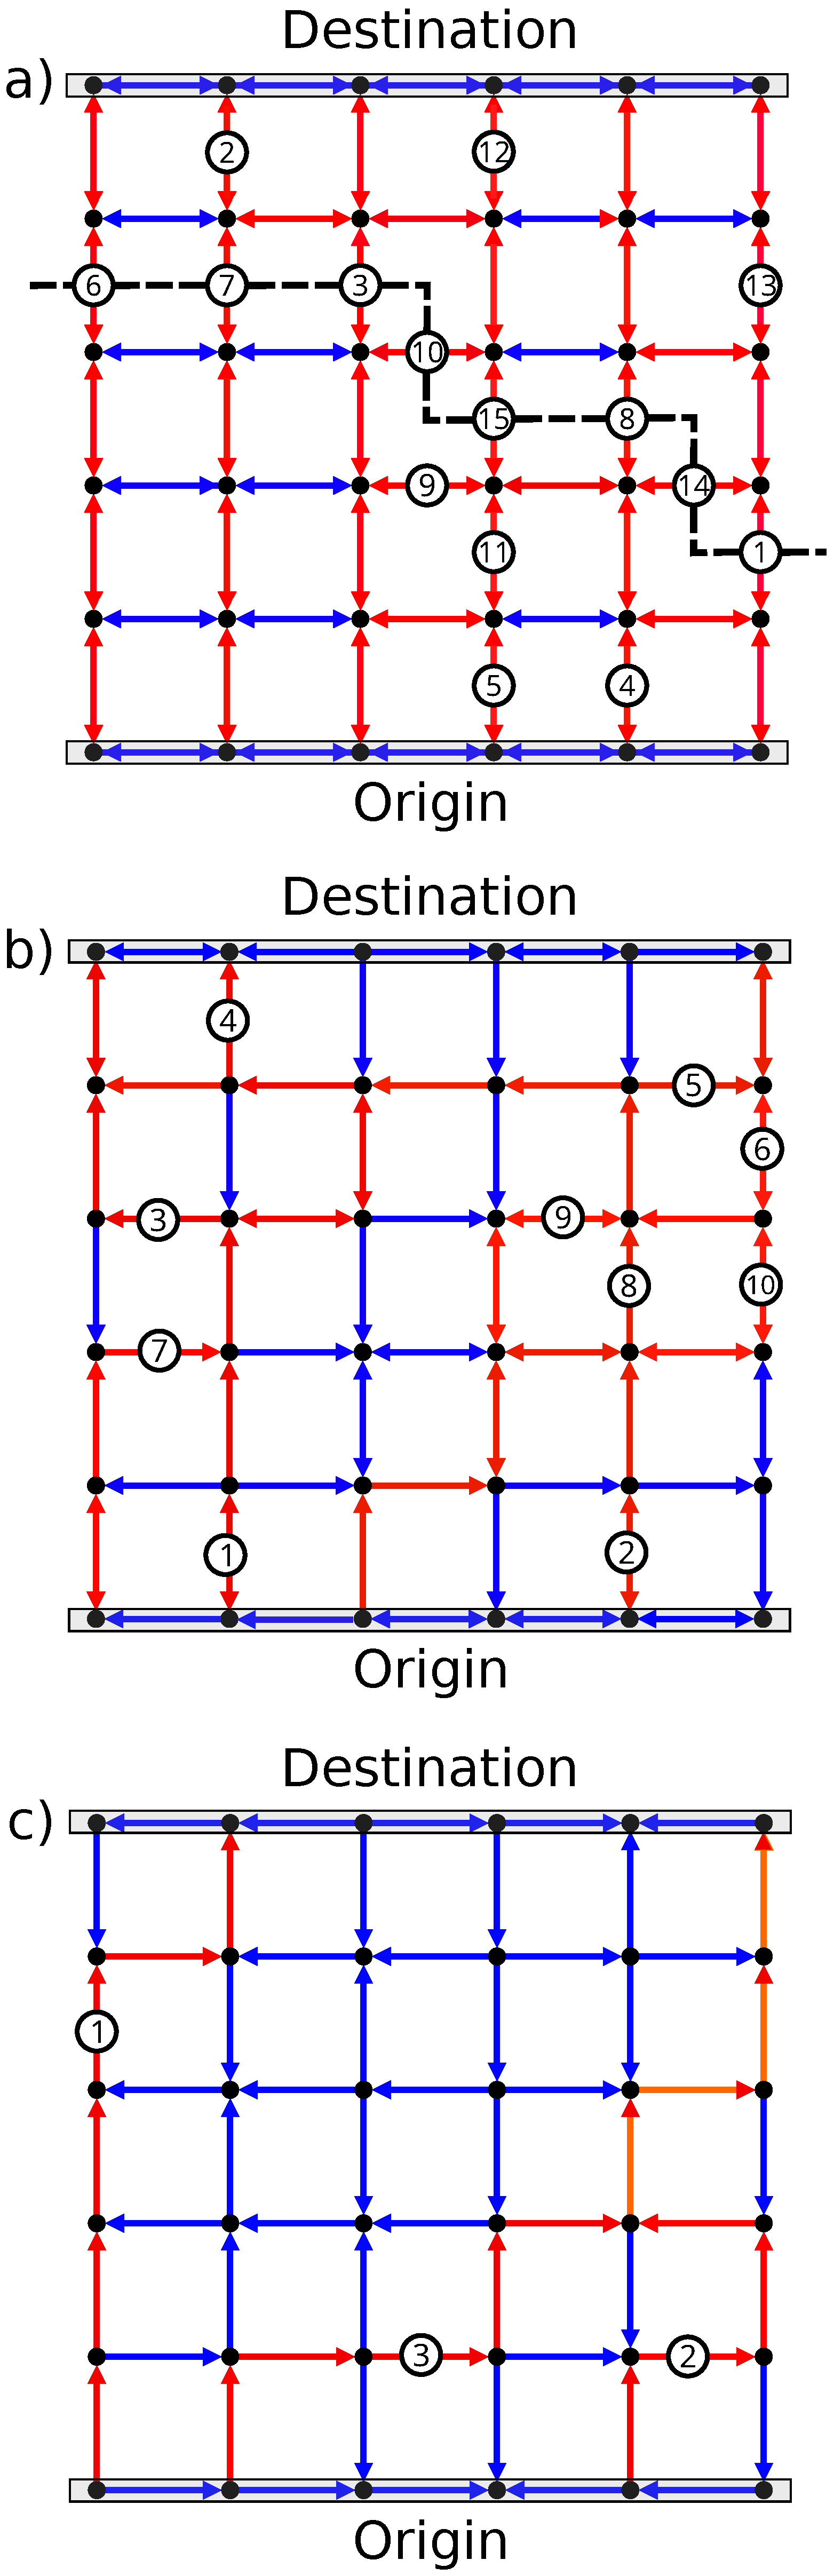
\includegraphics[width=0.57\columnwidth]{fig1} 
	\caption{Sequence of removed links during the OPC process for $6\times 6$
	square lattices under weak disorder in travelling times ($\beta=0.002$) and
	different values of the fraction $p$ of unidirectional links, namely, (a)
	$p=0$, (b) $p=0.4$, and (c) $p=1$. Before the collapse of the system, all links
	in red were part of an optimal path, at least once, from the bottom (origin) to
	the top (destination) of the lattice. Those removed are indicated with white
	circles in the middle, numbered according to the OPC removal sequence, as
	explained in the main text. The number of removed links clearly decreases with
	$p$. The dashed line in (a) corresponds to the fracture backbone that is always
	present as a result of the OPC process applied to fully bidirectional networks
	($p=0$)~\cite{Andrade2009}. ~\label{fig::spatial.distribution}}
\end{figure}
	
Without central planning, travellers usually choose the route that minimizes
their travelling time. However, when a road segment gets congested, a new
optimal route needs to be found. The optimal path crack model (OPC) was
introduced as a general framework to study the resilience of a network
infrastructure to a sequence of optimal path
failures~\cite{Andrade2009,Oliveira2011}. The OPC is described as follows. Let
us consider a square lattice of size $L$ with periodic boundary conditions in
the horizontal direction and fixed boundary conditions at the top and bottom. To
each link, a travelling time $t$ is randomly assigned according to a given
probability distribution $P(t)$, with $t>0$. Using Dijkstra's
algorithm~\cite{Dijkstra1959}, the first optimal path is identified which
minimizes the total travelling time between the bottom and the top of the
lattice. We then search and remove the most vulnerable link along this path,
defined as the one with the highest travelling time. The next optimal path is
identified, which cannot contain the removed link, and its vulnerable link is
also removed. We proceed iteratively until the lattice is disrupted and no more
paths can be found. The OPC is then the set of all removed links. In the limit
of strong disorder, all cracks are located on a single self-similar connected
line of fractal dimension equal to $1.22$~\cite{Andrade2009}. As
a matter of fact, this exponent value is statistically identical to the fractal
dimension previously found for the optimal path line under strong
disorder~\cite{Cieplak1994, Cieplak1996, Porto1997, Porto1999}, ``strands'' in
Invasion Percolation~\cite{Cieplak1994, Cieplak1996}, paths on Minimum Spanning
Trees~\cite{Dobrin2001}, and watersheds on uncorrelated
landscapes~\cite{Oliveira2011}. In the case of weak disorder, the cracks spread
all over the entire network before global connectivity is lost, so that the
total number of removed links scales as $N_{r} \sim L^{d}$, where $d$ is the
topological dimension of the lattice~\cite{Andrade2009}.

So far, all studies of OPC considered undirected networks. However, traffic
networks have a non-negligible fraction of one-way roads. For example, in
Manhattan and Boston about half of the roads are unidirectional. Here we first
perform simulations on square lattices in which the links are assigned to be
unidirectional with probability $p$ and bidirectional with probability $(1-p)$.
For $p=0$ we recover the OPC of a fully bidirectional lattice, while for $p=1$
all links are unidirectional. Disorder is introduced by assigning the travelling
times of unidirectional links according to a hyperbolic distribution
$p\left(\tau_i\right)\propto 1/\tau_i$, truncated between $\tau_{max}=1$ and
$\tau_{min} = \exp \left(-\beta\right)$, where $\beta \geq 0$ is the parameter
that controls the disorder. Note that, in general, each bidirectional link in the
network have distinct travelling times associated to its two directions. Typical
realizations of the OPC model for small networks generated with weak disorder
are shown in Fig.~\ref{fig::spatial.distribution}. As previously
observed~\cite{Andrade2009}, the set of OPC cracks generated in fully
bidirectional networks ($p=0$) always contains a contiguous subset that spans
the entire system from left to right, regardless of the level of disorder. In
the presence of any amount of unidirectional links ($p>0$), however, the cracks
do not necessarily form a contiguous fracture that divides the network into two
pieces. Moreover, the larger the value o $p$, more rare is the occurrence of
these spanning fractures.
	
Figure~\ref{fig::number.removed.links} shows the logarithmic dependence of the
number of removed links $N_r$ on the linear size of the lattice $L$, for
lattices with sizes varying in the range $16\leq L\leq 512$ and weak disorder in
their distribution of travelling times ($\beta=0.002$). For $p\neq 1$, the
numerical results are consistent with $N_r\sim L^d$, where $d=2$.  This result
suggests that, provided the lattice contains a non-zero fraction of
bidirectional links, the set of all removed links is compact, as reported
previously for regular lattices with only bidirectional links
($p=0$)~\cite{Andrade2009}. Nevertheless, the fraction of removed links is a
monotonic decreasing function of $p$ and so, the prefactor of the power-law
dependence decreases also with $p$ (see Fig.~\ref{fig::spatial.distribution}).
Surprisingly, in the limiting case of a completely unidirectional lattice,
$p=1$, we find that $N_r\sim L^{D_f}$, with $D_f=0.382\pm 0.002$. Our results
therefore indicate that the OPC set at this point belongs to a different
universality class. Moreover, since $D_f<d$, the fraction of removed links for
an infinite lattice (thermodynamic limit) is zero for $p=1$.
	
\begin{figure}[ht]
	\centering
	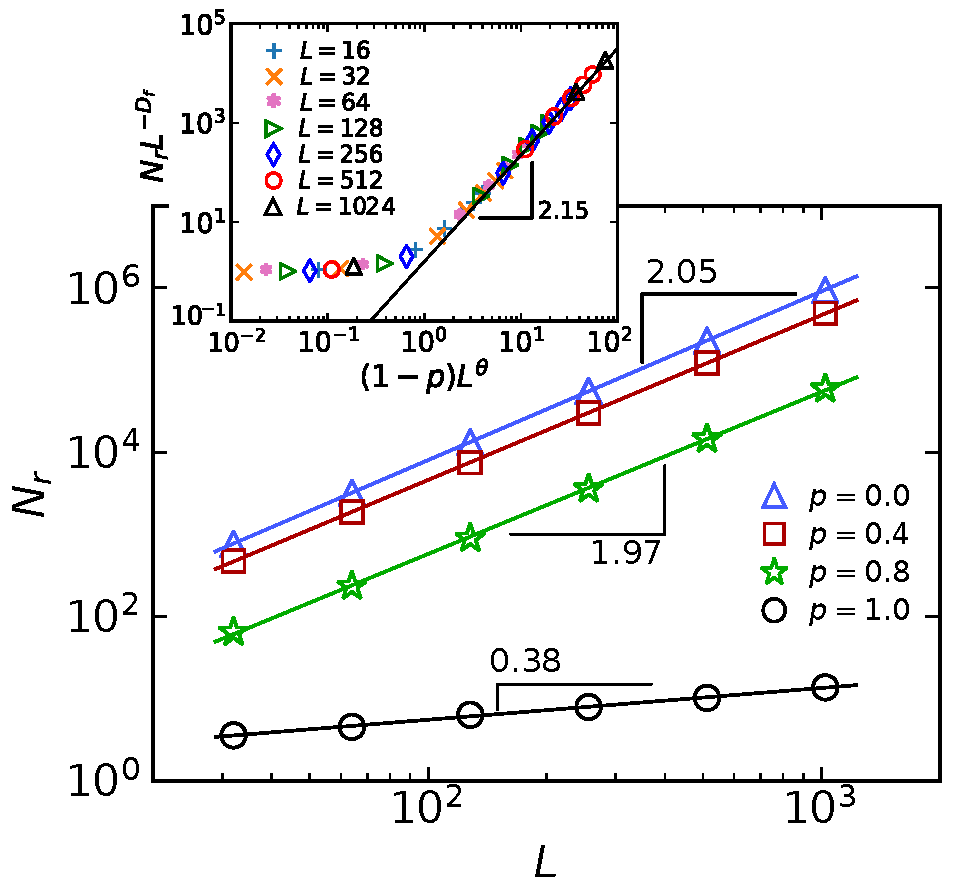
\includegraphics[width=0.85\columnwidth]{fig2} 
\caption{Logarithmic dependence of the total number of removed links $N_r$ on
	the linear size of the lattice $L$ for different values of the fraction $p$ of
	unidirectional links. The symbols correspond to averages over $100$ thousand
	network realizations and weak disorder in their traveling times
	($\beta=0.002$). The results for $p=0.4$ and $0.8$ are consistent with the
	scaling, $N_r\sim L^2$, obtained for $p=0$, namely, fully bidirectional
	lattices~\cite{Andrade2009}. For a completely unidirectional lattice, $p=1$, we
	find that $N_r\sim L^{D_f}$, with $D_f=0.382\pm 0.002$. The error bars are
	smaller than the symbols. The inset shows the tricritical crossover scaling and
	data collapse for the OPC model on regular lattices. The scaling function is
	given by Eq.~\eqref{eq::ansatz}, with $D_f=0.38$ and $\theta=0.753$. The solid
	line in the inset represents a power law with exponent $2.15$.
	~\label{fig::number.removed.links}}
\end{figure}


	
\begin{figure}[ht]
	\centering
	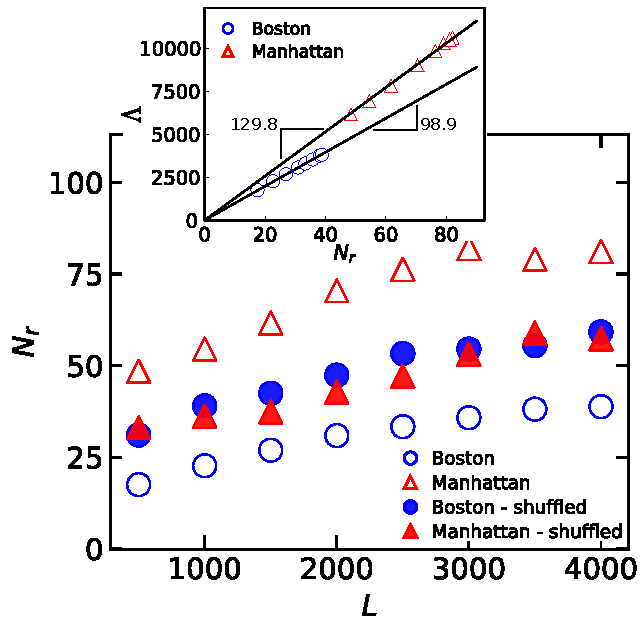
\includegraphics[width=0.85\columnwidth]{fig3} 
    \caption{Dependence of the total number of removed roads $N_r$ on the
	origin-destination distance $L$ (in meters) for downtown Boston and
	Manhattan (open symbols). Numerical results are averages over 2000 OD
	samples for each city. Also shown  are the results of OPC simulations
	preserving the geometry of the road networks, but shuffling the values of
	$t/\ell$ among randomly chosen pairs of road segments (filled symbols). The
	inset shows the linear dependence, $\Lambda=a N_r$, with $a=98.9 \pm 0.03$
	and $129.8\pm 0.04$ for Boston and Manhattan, respectively. In all cases,
	the error bars are smaller than the symbols.~\label{fig::real.data}}
\end{figure} 


\begin{figure*}[ht] 
	\centering
	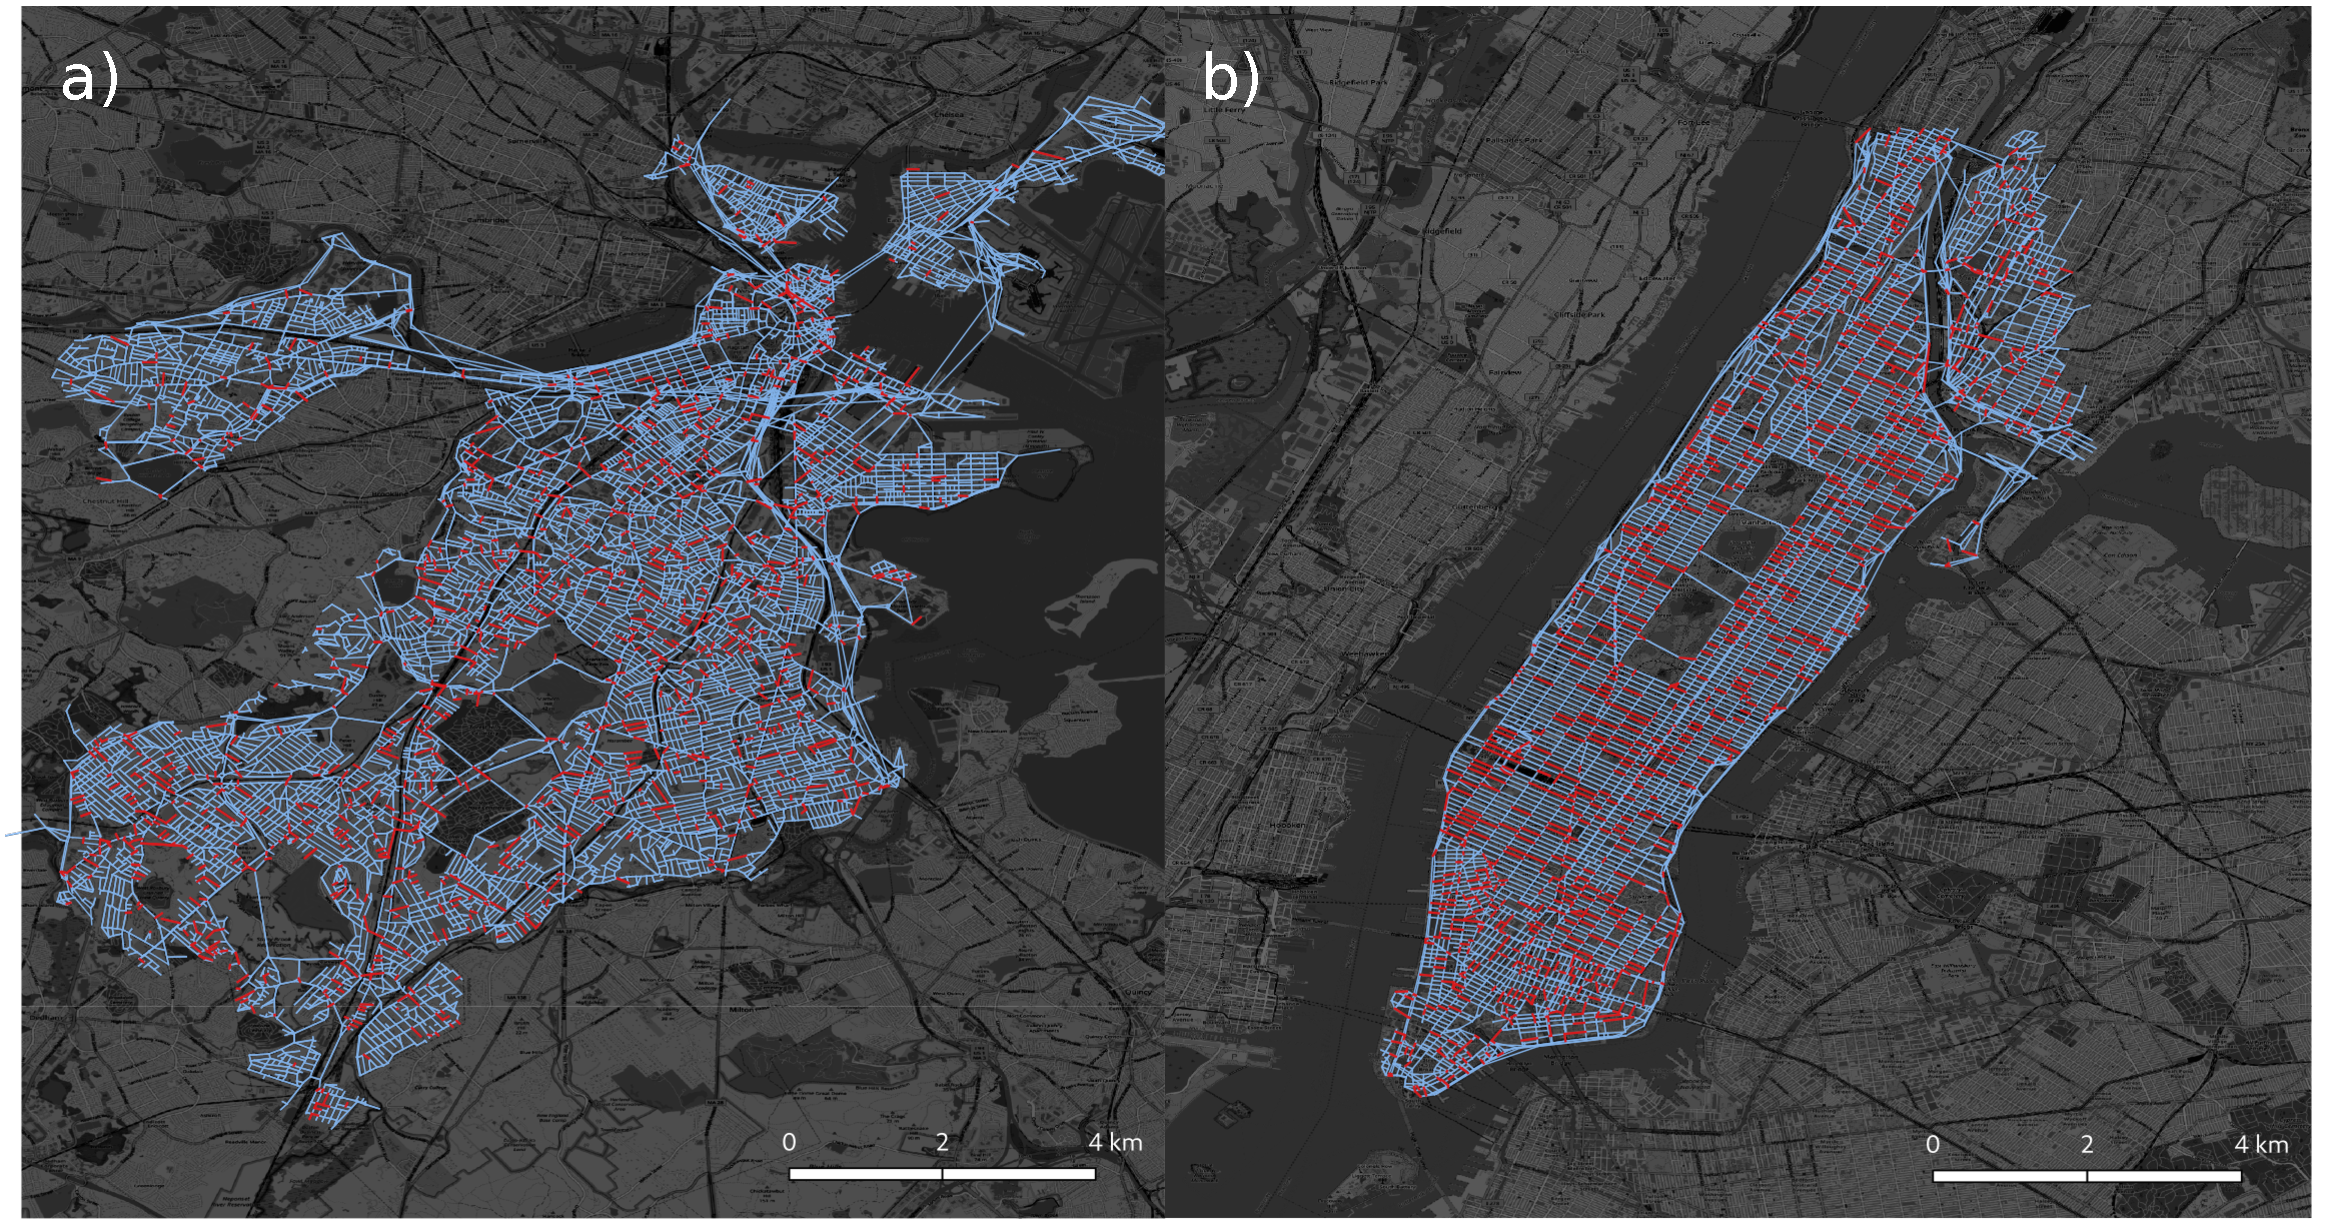
\includegraphics[width=0.7\textwidth]{fig4.pdf}
	\caption{Road maps for downtown Boston (left) and Manhattan (right). The thick
	red lines are the road segments that have been removed first. All other road
	segments are shown in blue. Only OPC samples performed with OD distances
	$L=2000$ m have been considered.~\label{fig::real.data.maps}}
\end{figure*} %


The statistics of the OPC set generated under weak disorder suggests that its
dimension does crossover from $d$, for $p>1$, to $D_f$ at $p=1$. This crossover
is analogous to what is observed at the theta point of polymer
systems~\cite{deGennes1979,Chang1991,Poole1989}. At high temperatures, the
configurations of a polymer chain are well described by a self-avoiding random
walk, as the only relevant interactions are excluded volume. However, at the
theta-temperature, the attractive forces are no longer negligible, and the
statistics are then different. Also, in ranked surfaces, when occupying links
sequentially, but suppressing global connectivity, the fractal dimension of the
set of links that are not occupied due to this constraint changes from $3/4$ at
the percolation threshold to $1.22$ above it~\cite{Schrenk2012}. For the case of
OPC, we consider the following crossover \textit{Ansatz}:
%
\begin{equation}
	\label{eq::ansatz}
	N_r=L^D\mathcal{F}\left[\left(p-p_c\right)L^\theta\right],
\end{equation} 
%
where $\theta$ is the crossover exponent, $\mathcal{F}\left[x\right]\sim
x^{\eta}$ for $x\neq0$ and equal to a nonzero constant at $x=0$. The inset
in Fig.~\ref{fig::number.removed.links} shows the data collapse obtained
with this tricritical scaling for different lattice sizes and values of
$p$, with $\theta=0.753$. By fitting the power-law regime of the scaling
function $\mathcal{F}$, we estimate $\eta=2.15\pm0.03$. From the
\textit{Ansatz}, we expect that, 
%
\begin{equation}\label{eq::exponents} %
	D_f+\eta\theta=d, %
\end{equation} 
%
what is verified, within error bars. This behavior confirms that the
universality class of OPC is robust and only breaks down for a fully
unidirectional lattice ($p=1$).
	
For the case of local travelling times with strong disorder, $\beta=400$
(see Fig.~S1 of the Supplemental Material), the
OPC results for $p\neq 1$ are consistent with the behavior previously
observed for fully bidirectional networks ($p=0$), namely, $D_{f}=1.22\pm
0.01$~\cite{Andrade2009}. As in the weak disorder case, it is only for
$p=1$ that the finite-size scaling of the system becomes noticeably
different, with $D_f=0.002\pm 0.004$. A rather small number of removed links
is therefore sufficient to block a fully directed lattice subjected to
strong disorder.
     
Next, we show that the OPC can be effectively used as a proxy for urban mobility. 
%Strictly speaking, this model represents a dynamic process
%and the resulting set of ``cracks'' necessary to block a given road network
%should only depend on its intrinsic topology as well as on the distribution
%of travelling times associated with their elementary segments. 
In general, the fraction of one-way roads changes from city to city. Here we
apply the OPC method to two metropolitan areas in US, namely, Manhattan and
downtown Boston, the latter being the top one in the rank of North America for
average time waste in traffic~\cite{GlobalTrafficReport2018}. For this purpose,
we obtained the road network structures of both urban areas from
OpenStreetMap~\cite{OpenStreetMap}. Their corresponding average travelling times
per road were downloaded from Directions API Google~\cite{GoogleDirections},
specifically for November 21th of 2018 at 4:00 am. This off-peak data set has
been chosen because, by construction, the travelling times should somehow
reflect the freeway-state of the streets and avenues constituting a given urban
mobility system. In order to assess the efficiency of these road networks to
urban traffic, the OPC is numerically calculated for different pairs of
origin-destination (OD) sites. Precisely, for each OPC realization, one site of
the network is selected at random to be the center of a circle of radius $L$. A
point on this circle is then randomly chosen and the closest road sites to the
center and to this point are taken as the origin and destination, respectively,
only if the distance between them is equal to $L$ within a tolerance of $5\%$.
Here, due to the fact that road segments composing the urban networks have
different travelling times $t$ as well as lengths $\ell$, an optimal path is
identified among all possible paths during the OPC process as the one with the
minimum sum of $t/\ell$ over all its road segments.
	
OPC simulations have then been performed with $2000$ OD realizations for Boston
and Manhattan. One should note that the bidirectional links (two-way streets and
avenues) are in fact composed of two unidirectional ones of contrary directions
that can be removed independently during the OPC process. 
%In this way, every bidirectional link has to become unidirectional before being
%completely removed from the network.
In Fig.~\ref{fig::real.data}, we show how the average number of removed sites
$N_r$ varies with the distance $L$ for both urban areas. The smaller $N_r$ is,
less resilient is the road network. These results indicate that Boston is
systematically much more vulnerable than Manhattan, regardless of the
origin-destination distance $L$, what is consistent with their relative
positions in the national rank of urban mobility. Moreover, the same behavior
can be observed if, instead of $N_r$, we quantify the result of each OPC process
in terms of the sum $\Lambda=\sum_{i=1}^{N_r}\lambda$, where $\lambda$ is equal
to the length $\ell$ of the removed road segment at iteration $i$.
Interestingly, as shown in the inset of Fig.~\ref{fig::real.data}, these two
measures are, in fact, linearly related $\left<\Lambda\right>=a N_r$, with $a =
98.9\,\rm{m}$ and $129.8\,\rm{m}$ for Boston and Manhattan, respectively. For
all practical purposes, this indicates the absence of statistical correlations
in the OPC process of selecting $\lambda$ from the distribution of segment
lengths $P(\ell)$ of both road networks. The similarities between distributions
$P(\ell)$ and $P(\lambda)$ for Boston and Manhattan are compatible with this
argument (see Fig.~S2 of Supplemental Material).

The modest differences in the distributions $P(t/\ell)$ obtained for Boston and
Manhattan (see Fig.~S3 of the Supplemental Material) are not compatible
with such a striking discrepancy in their resilience. One therefore can only
rely on the particular features of the intrinsic spatial correlations that
should be present in these urban systems to justify their very distinct
responses. In order to test for this hypothesis, we performed additional OPC
simulations preserving the geometry of both networks, but shuffling the values
of $t/\ell$ among randomly chosen pairs of road segments. The results presented
in Fig.~\ref{fig::real.data} are rather surprising and twofold. First, they show
that the effect of suppressing the spatial correlations is to practically
collapse the curves $N_r$ against $L$ of both cities to a single curve,
therefore demonstrating the generality and comparative power of the OPC method
for urban mobility. Second, the fact that the values of $N_r$ systematically
increase for Boston and decrease for Manhattan, as compared to the results using
the real (non-shuffled) data sets, corroborates the ability of our approach to
properly capture negative and positive effects of spatial correlations on urban
mobility.
	
One question that naturally arises is how the OPC method can be used to enhance
urban mobility. A possible answer is to prioritize rerouting and structural
improvements based on the identification of those road segments that are more
frequently appearing among the first removals in all OPC sequences. In
Fig.~\ref{fig::real.data.maps} are the road maps for the two urban areas, where
the highlighted road segments (thick and red) correspond to all those removed
first, considering all OPC samples performed with OD distances $L=2000$ m. For
downtown Boston, we find that only a percentage of $5.4\%$ of all road segments
is removed, while $10.0\%$ is the value for Manhattan. The cumulative dependence
of the percentage of all first removals on the percentage of the most frequent
ones is shown in Fig.~S4 of the Supplemental Material. These results suggest
that, as compared to Manhattan, a relatively small number of potential local
changes in Boston might be very efficient in improving urban mobility. The fact
that Manhattan is much more resilient should therefore increase the costs of
improvements.

In summary, we proposed a proxy for resilience of urban mobility based on OPC.
Our results with synthetic and real road networks suggest that their
vulnerability to traffic congestion are strongly dependent on the level of
disorder, fraction of unidirectional segments and intrinsic spatial
correlations. These observations have practical implications in the design and
restructuring for improved urban mobility. We conclude that OPC is a general and
powerful method to access urban mobility, and gives practical insight that can
effectively help identifying and mitigating vulnerabilities of real road
networks.

\begin{acknowledgments}  
%
We acknowledge financial support from the Brazilian agencies CNPq, CAPES
and FUNCAP, and from the Portuguese Foundation for Science and Technology
(FCT) under Contracts no. UIDB/00618/2020 and UIDP/00618/2020. 
%
\end{acknowledgments}
%\bibliography{references.bib}
\begin{thebibliography}{30}%
	\makeatletter
	\providecommand \@ifxundefined [1]{%
	 \@ifx{#1\undefined}
	}%
	\providecommand \@ifnum [1]{%
	 \ifnum #1\expandafter \@firstoftwo
	 \else \expandafter \@secondoftwo
	 \fi
	}%
	\providecommand \@ifx [1]{%
	 \ifx #1\expandafter \@firstoftwo
	 \else \expandafter \@secondoftwo
	 \fi
	}%
	\providecommand \natexlab [1]{#1}%
	\providecommand \enquote  [1]{``#1''}%
	\providecommand \bibnamefont  [1]{#1}%
	\providecommand \bibfnamefont [1]{#1}%
	\providecommand \citenamefont [1]{#1}%
	\providecommand \href@noop [0]{\@secondoftwo}%
	\providecommand \href [0]{\begingroup \@sanitize@url \@href}%
	\providecommand \@href[1]{\@@startlink{#1}\@@href}%
	\providecommand \@@href[1]{\endgroup#1\@@endlink}%
	\providecommand \@sanitize@url [0]{\catcode `\\12\catcode `\$12\catcode
	  `\&12\catcode `\#12\catcode `\^12\catcode `\_12\catcode `\%12\relax}%
	\providecommand \@@startlink[1]{}%
	\providecommand \@@endlink[0]{}%
	\providecommand \url  [0]{\begingroup\@sanitize@url \@url }%
	\providecommand \@url [1]{\endgroup\@href {#1}{\urlprefix }}%
	\providecommand \urlprefix  [0]{URL }%
	\providecommand \Eprint [0]{\href }%
	\providecommand \doibase [0]{http://dx.doi.org/}%
	\providecommand \selectlanguage [0]{\@gobble}%
	\providecommand \bibinfo  [0]{\@secondoftwo}%
	\providecommand \bibfield  [0]{\@secondoftwo}%
	\providecommand \translation [1]{[#1]}%
	\providecommand \BibitemOpen [0]{}%
	\providecommand \bibitemStop [0]{}%
	\providecommand \bibitemNoStop [0]{.\EOS\space}%
	\providecommand \EOS [0]{\spacefactor3000\relax}%
	\providecommand \BibitemShut  [1]{\csname bibitem#1\endcsname}%
	\let\auto@bib@innerbib\@empty
	%</preamble>
	\bibitem [{\citenamefont {Reed}\ and\ \citenamefont
	  {Kidd}(2018)}]{GlobalTrafficReport2018}%
	  \BibitemOpen
	  \bibfield  {author} {\bibinfo {author} {\bibfnamefont {T.}~\bibnamefont
	  {Reed}}\ and\ \bibinfo {author} {\bibfnamefont {J.}~\bibnamefont {Kidd}},\
	  }\href@noop {} {\emph {\bibinfo {title} {INRIX Global Traffic Scorecard
	  2018}}},\ \bibinfo {type} {Tech. Rep.}\ (\bibinfo  {institution} {IRIX
	  Research, United States},\ \bibinfo {year} {2018})\BibitemShut {NoStop}%
	\bibitem [{\citenamefont {Sweet}(2014)}]{Sweet2014}%
	  \BibitemOpen
	  \bibfield  {author} {\bibinfo {author} {\bibfnamefont {M.}~\bibnamefont
	  {Sweet}},\ }\href@noop {} {\bibfield  {journal} {\bibinfo  {journal} {Urban
	  Studies}\ }\textbf {\bibinfo {volume} {51}},\ \bibinfo {pages} {2088}
	  (\bibinfo {year} {2014})}\BibitemShut {NoStop}%
	\bibitem [{\citenamefont {Louf}\ and\ \citenamefont
	  {Barthelemy}(2014)}]{Louf2014}%
	  \BibitemOpen
	  \bibfield  {author} {\bibinfo {author} {\bibfnamefont {R.}~\bibnamefont
	  {Louf}}\ and\ \bibinfo {author} {\bibfnamefont {M.}~\bibnamefont
	  {Barthelemy}},\ }\href@noop {} {\bibfield  {journal} {\bibinfo  {journal}
	  {Sci. Rep.}\ }\textbf {\bibinfo {volume} {4}},\ \bibinfo {pages} {1}
	  (\bibinfo {year} {2014})}\BibitemShut {NoStop}%
	\bibitem [{\citenamefont {Colak}\ \emph {et~al.}(2016)\citenamefont {Colak},
	  \citenamefont {Lima},\ and\ \citenamefont {Gonz{\'{a}}lez}}]{Colak2016}%
	  \BibitemOpen
	  \bibfield  {author} {\bibinfo {author} {\bibfnamefont {S.}~\bibnamefont
	  {Colak}}, \bibinfo {author} {\bibfnamefont {A.}~\bibnamefont {Lima}}, \ and\
	  \bibinfo {author} {\bibfnamefont {M.~C.}\ \bibnamefont {Gonz{\'{a}}lez}},\
	  }\href@noop {} {\bibfield  {journal} {\bibinfo  {journal} {Nat. Commun.}\
	  }\textbf {\bibinfo {volume} {7}},\ \bibinfo {pages} {10793} (\bibinfo {year}
	  {2016})}\BibitemShut {NoStop}%
	\bibitem [{\citenamefont {Sol{\'{e}}-Ribalta}\ \emph
	  {et~al.}(2018)\citenamefont {Sol{\'{e}}-Ribalta}, \citenamefont
	  {G{\'{o}}mez},\ and\ \citenamefont {Arenas}}]{Sole-Ribalta2018}%
	  \BibitemOpen
	  \bibfield  {author} {\bibinfo {author} {\bibfnamefont {A.}~\bibnamefont
	  {Sol{\'{e}}-Ribalta}}, \bibinfo {author} {\bibfnamefont {S.}~\bibnamefont
	  {G{\'{o}}mez}}, \ and\ \bibinfo {author} {\bibfnamefont {A.}~\bibnamefont
	  {Arenas}},\ }\href@noop {} {\bibfield  {journal} {\bibinfo  {journal}
	  {Networks Spat. Econ.}\ }\textbf {\bibinfo {volume} {18}},\ \bibinfo {pages}
	  {33} (\bibinfo {year} {2018})}\BibitemShut {NoStop}%
	\bibitem [{\citenamefont {Barbosa}\ \emph {et~al.}(2018)\citenamefont
	  {Barbosa}, \citenamefont {Barthelemy}, \citenamefont {Ghoshal}, \citenamefont
	  {James}, \citenamefont {Lenormand}, \citenamefont {Louail}, \citenamefont
	  {Menezes}, \citenamefont {Ramasco}, \citenamefont {Simini},\ and\
	  \citenamefont {Tomasini}}]{Barbosa2018}%
	  \BibitemOpen
	  \bibfield  {author} {\bibinfo {author} {\bibfnamefont {H.}~\bibnamefont
	  {Barbosa}}, \bibinfo {author} {\bibfnamefont {M.}~\bibnamefont {Barthelemy}},
	  \bibinfo {author} {\bibfnamefont {G.}~\bibnamefont {Ghoshal}}, \bibinfo
	  {author} {\bibfnamefont {C.~R.}\ \bibnamefont {James}}, \bibinfo {author}
	  {\bibfnamefont {M.}~\bibnamefont {Lenormand}}, \bibinfo {author}
	  {\bibfnamefont {T.}~\bibnamefont {Louail}}, \bibinfo {author} {\bibfnamefont
	  {R.}~\bibnamefont {Menezes}}, \bibinfo {author} {\bibfnamefont {J.~J.}\
	  \bibnamefont {Ramasco}}, \bibinfo {author} {\bibfnamefont {F.}~\bibnamefont
	  {Simini}}, \ and\ \bibinfo {author} {\bibfnamefont {M.}~\bibnamefont
	  {Tomasini}},\ }\href@noop {} {\bibfield  {journal} {\bibinfo  {journal}
	  {Phys. Rep.}\ }\textbf {\bibinfo {volume} {734}},\ \bibinfo {pages} {1}
	  (\bibinfo {year} {2018})}\BibitemShut {NoStop}%
	\bibitem [{\citenamefont {Barthelemy}(2019)}]{Barthelemy2019}%
	  \BibitemOpen
	  \bibfield  {author} {\bibinfo {author} {\bibfnamefont {M.}~\bibnamefont
	  {Barthelemy}},\ }\href@noop {} {\bibfield  {journal} {\bibinfo  {journal}
	  {Nature Reviews Physics}\ }\textbf {\bibinfo {volume} {1}},\ \bibinfo {pages}
	  {406} (\bibinfo {year} {2019})}\BibitemShut {NoStop}%
	\bibitem [{\citenamefont {Li}\ \emph {et~al.}(2015)\citenamefont {Li},
	  \citenamefont {Fu}, \citenamefont {Wang}, \citenamefont {Lu}, \citenamefont
	  {Berezin}, \citenamefont {Stanley},\ and\ \citenamefont {Havlin}}]{Li2015}%
	  \BibitemOpen
	  \bibfield  {author} {\bibinfo {author} {\bibfnamefont {D.}~\bibnamefont
	  {Li}}, \bibinfo {author} {\bibfnamefont {B.}~\bibnamefont {Fu}}, \bibinfo
	  {author} {\bibfnamefont {Y.}~\bibnamefont {Wang}}, \bibinfo {author}
	  {\bibfnamefont {G.}~\bibnamefont {Lu}}, \bibinfo {author} {\bibfnamefont
	  {Y.}~\bibnamefont {Berezin}}, \bibinfo {author} {\bibfnamefont {H.~E.}\
	  \bibnamefont {Stanley}}, \ and\ \bibinfo {author} {\bibfnamefont
	  {S.}~\bibnamefont {Havlin}},\ }\href@noop {} {\bibfield  {journal} {\bibinfo
	  {journal} {Proc. Natl. Acad. Sci. U. S. A.}\ }\textbf {\bibinfo {volume}
	  {112}},\ \bibinfo {pages} {669} (\bibinfo {year} {2015})}\BibitemShut
	  {NoStop}%
	\bibitem [{\citenamefont {Gonz{\'{a}}lez}\ \emph {et~al.}(2008)\citenamefont
	  {Gonz{\'{a}}lez}, \citenamefont {Hidalgo},\ and\ \citenamefont
	  {Barab{\'{a}}si}}]{Gonzalez2008}%
	  \BibitemOpen
	  \bibfield  {author} {\bibinfo {author} {\bibfnamefont {M.~C.}\ \bibnamefont
	  {Gonz{\'{a}}lez}}, \bibinfo {author} {\bibfnamefont {C.~A.}\ \bibnamefont
	  {Hidalgo}}, \ and\ \bibinfo {author} {\bibfnamefont {A.-L.}\ \bibnamefont
	  {Barab{\'{a}}si}},\ }\href@noop {} {\bibfield  {journal} {\bibinfo  {journal}
	  {Nature}\ }\textbf {\bibinfo {volume} {453}},\ \bibinfo {pages} {779}
	  (\bibinfo {year} {2008})}\BibitemShut {NoStop}%
	\bibitem [{\citenamefont {Olmos}\ \emph {et~al.}(2018)\citenamefont {Olmos},
	  \citenamefont {{\c{C}}olak}, \citenamefont {Shafiei}, \citenamefont
	  {Saberi},\ and\ \citenamefont {Gonz{\'{a}}lez}}]{Olmos2018}%
	  \BibitemOpen
	  \bibfield  {author} {\bibinfo {author} {\bibfnamefont {L.~E.}\ \bibnamefont
	  {Olmos}}, \bibinfo {author} {\bibfnamefont {S.}~\bibnamefont {{\c{C}}olak}},
	  \bibinfo {author} {\bibfnamefont {S.}~\bibnamefont {Shafiei}}, \bibinfo
	  {author} {\bibfnamefont {M.}~\bibnamefont {Saberi}}, \ and\ \bibinfo {author}
	  {\bibfnamefont {M.~C.}\ \bibnamefont {Gonz{\'{a}}lez}},\ }\href@noop {}
	  {\bibfield  {journal} {\bibinfo  {journal} {Proc. Natl. Acad. Sci. U. S. A.}\
	  }\textbf {\bibinfo {volume} {115}},\ \bibinfo {pages} {12654} (\bibinfo
	  {year} {2018})}\BibitemShut {NoStop}%
	\bibitem [{\citenamefont {Zeng}\ \emph {et~al.}(2019)\citenamefont {Zeng},
	  \citenamefont {Li}, \citenamefont {Guo}, \citenamefont {Gao}, \citenamefont
	  {Gao}, \citenamefont {{Eugene Stanley}},\ and\ \citenamefont
	  {Havlin}}]{Zeng2019}%
	  \BibitemOpen
	  \bibfield  {author} {\bibinfo {author} {\bibfnamefont {G.}~\bibnamefont
	  {Zeng}}, \bibinfo {author} {\bibfnamefont {D.}~\bibnamefont {Li}}, \bibinfo
	  {author} {\bibfnamefont {S.}~\bibnamefont {Guo}}, \bibinfo {author}
	  {\bibfnamefont {L.}~\bibnamefont {Gao}}, \bibinfo {author} {\bibfnamefont
	  {Z.}~\bibnamefont {Gao}}, \bibinfo {author} {\bibfnamefont {H.}~\bibnamefont
	  {{Eugene Stanley}}}, \ and\ \bibinfo {author} {\bibfnamefont
	  {S.}~\bibnamefont {Havlin}},\ }\href@noop {} {\bibfield  {journal} {\bibinfo
	  {journal} {Proc. Natl. Acad. Sci. U. S. A.}\ }\textbf {\bibinfo {volume}
	  {116}},\ \bibinfo {pages} {23} (\bibinfo {year} {2019})}\BibitemShut
	  {NoStop}%
	\bibitem [{\citenamefont {Zhu}\ and\ \citenamefont {Levinson}(2015)}]{Zhu2015}%
	  \BibitemOpen
	  \bibfield  {author} {\bibinfo {author} {\bibfnamefont {S.}~\bibnamefont
	  {Zhu}}\ and\ \bibinfo {author} {\bibfnamefont {D.}~\bibnamefont {Levinson}},\
	  }\href@noop {} {\bibfield  {journal} {\bibinfo  {journal} {PLoS One}\
	  }\textbf {\bibinfo {volume} {10}},\ \bibinfo {pages} {e0134322} (\bibinfo
	  {year} {2015})}\BibitemShut {NoStop}%
	\bibitem [{\citenamefont {Lima}\ \emph {et~al.}(2016)\citenamefont {Lima},
	  \citenamefont {Stanojevic}, \citenamefont {Papagiannaki}, \citenamefont
	  {Rodriguez},\ and\ \citenamefont {Gonzalez}}]{Lima2016}%
	  \BibitemOpen
	  \bibfield  {author} {\bibinfo {author} {\bibfnamefont {A.}~\bibnamefont
	  {Lima}}, \bibinfo {author} {\bibfnamefont {R.}~\bibnamefont {Stanojevic}},
	  \bibinfo {author} {\bibfnamefont {D.}~\bibnamefont {Papagiannaki}}, \bibinfo
	  {author} {\bibfnamefont {P.}~\bibnamefont {Rodriguez}}, \ and\ \bibinfo
	  {author} {\bibfnamefont {M.~C.}\ \bibnamefont {Gonzalez}},\ }\href@noop {}
	  {\bibfield  {journal} {\bibinfo  {journal} {J. R. Soc. Interface}\ }\textbf
	  {\bibinfo {volume} {13}} (\bibinfo {year} {2016})}\BibitemShut {NoStop}%
	\bibitem [{\citenamefont {Zhang}\ \emph {et~al.}(2019)\citenamefont {Zhang},
	  \citenamefont {Zeng}, \citenamefont {Li}, \citenamefont {Huang},
	  \citenamefont {{Eugene Stanley}},\ and\ \citenamefont {Havlin}}]{Zhang2019}%
	  \BibitemOpen
	  \bibfield  {author} {\bibinfo {author} {\bibfnamefont {L.}~\bibnamefont
	  {Zhang}}, \bibinfo {author} {\bibfnamefont {G.}~\bibnamefont {Zeng}},
	  \bibinfo {author} {\bibfnamefont {D.}~\bibnamefont {Li}}, \bibinfo {author}
	  {\bibfnamefont {H.~J.}\ \bibnamefont {Huang}}, \bibinfo {author}
	  {\bibfnamefont {H.}~\bibnamefont {{Eugene Stanley}}}, \ and\ \bibinfo
	  {author} {\bibfnamefont {S.}~\bibnamefont {Havlin}},\ }\href@noop {}
	  {\bibfield  {journal} {\bibinfo  {journal} {Proc. Natl. Acad. Sci. U. S. A.}\
	  }\textbf {\bibinfo {volume} {116}},\ \bibinfo {pages} {8673} (\bibinfo {year}
	  {2019})}\BibitemShut {NoStop}%
	\bibitem [{\citenamefont {Wang}\ \emph {et~al.}(2012)\citenamefont {Wang},
	  \citenamefont {Hunter}, \citenamefont {Bayen}, \citenamefont {Schechtner},\
	  and\ \citenamefont {Gonz{\'{a}}lez}}]{Wang2012}%
	  \BibitemOpen
	  \bibfield  {author} {\bibinfo {author} {\bibfnamefont {P.}~\bibnamefont
	  {Wang}}, \bibinfo {author} {\bibfnamefont {T.}~\bibnamefont {Hunter}},
	  \bibinfo {author} {\bibfnamefont {A.~M.}\ \bibnamefont {Bayen}}, \bibinfo
	  {author} {\bibfnamefont {K.}~\bibnamefont {Schechtner}}, \ and\ \bibinfo
	  {author} {\bibfnamefont {M.~C.}\ \bibnamefont {Gonz{\'{a}}lez}},\ }\href@noop
	  {} {\bibfield  {journal} {\bibinfo  {journal} {Sci. Rep.}\ }\textbf {\bibinfo
	  {volume} {2}},\ \bibinfo {pages} {1001} (\bibinfo {year} {2012})}\BibitemShut
	  {NoStop}%
	\bibitem [{\citenamefont {Guo}\ \emph {et~al.}(2019)\citenamefont {Guo},
	  \citenamefont {Zhou}, \citenamefont {Fan}, \citenamefont {Tong},
	  \citenamefont {Zhu}, \citenamefont {Lv}, \citenamefont {Li},\ and\
	  \citenamefont {Havlin}}]{Guo2019}%
	  \BibitemOpen
	  \bibfield  {author} {\bibinfo {author} {\bibfnamefont {S.}~\bibnamefont
	  {Guo}}, \bibinfo {author} {\bibfnamefont {D.}~\bibnamefont {Zhou}}, \bibinfo
	  {author} {\bibfnamefont {J.}~\bibnamefont {Fan}}, \bibinfo {author}
	  {\bibfnamefont {Q.}~\bibnamefont {Tong}}, \bibinfo {author} {\bibfnamefont
	  {T.}~\bibnamefont {Zhu}}, \bibinfo {author} {\bibfnamefont {W.}~\bibnamefont
	  {Lv}}, \bibinfo {author} {\bibfnamefont {D.}~\bibnamefont {Li}}, \ and\
	  \bibinfo {author} {\bibfnamefont {S.}~\bibnamefont {Havlin}},\ }\href@noop {}
	  {\bibfield  {journal} {\bibinfo  {journal} {EPJ Data Sci.}\ }\textbf
	  {\bibinfo {volume} {8}},\ \bibinfo {pages} {28} (\bibinfo {year}
	  {2019})}\BibitemShut {NoStop}%
	\bibitem [{\citenamefont {\mbox{Andrade Jr}}\ \emph {et~al.}(2009)\citenamefont
	  {\mbox{Andrade Jr}}, \citenamefont {Oliveira}, \citenamefont {Moreira},\ and\
	  \citenamefont {Herrmann}}]{Andrade2009}%
	  \BibitemOpen
	  \bibfield  {author} {\bibinfo {author} {\bibfnamefont {J.~S.}\ \bibnamefont
	  {\mbox{Andrade Jr}}}, \bibinfo {author} {\bibfnamefont {E.~A.}\ \bibnamefont
	  {Oliveira}}, \bibinfo {author} {\bibfnamefont {A.~A.}\ \bibnamefont
	  {Moreira}}, \ and\ \bibinfo {author} {\bibfnamefont {H.~J.}\ \bibnamefont
	  {Herrmann}},\ }\href@noop {} {\bibfield  {journal} {\bibinfo  {journal}
	  {Phys. Rev. Lett.}\ }\textbf {\bibinfo {volume} {103}},\ \bibinfo {pages}
	  {225503} (\bibinfo {year} {2009})}\BibitemShut {NoStop}%
	\bibitem [{\citenamefont {Oliveira}\ \emph {et~al.}(2011)\citenamefont
	  {Oliveira}, \citenamefont {Schrenk}, \citenamefont {Araújo}, \citenamefont
	  {Herrmann},\ and\ \citenamefont {Andrade}}]{Oliveira2011}%
	  \BibitemOpen
	  \bibfield  {author} {\bibinfo {author} {\bibfnamefont {E.~A.}\ \bibnamefont
	  {Oliveira}}, \bibinfo {author} {\bibfnamefont {K.~J.}\ \bibnamefont
	  {Schrenk}}, \bibinfo {author} {\bibfnamefont {N.~A.~M.}\ \bibnamefont
	  {Araújo}}, \bibinfo {author} {\bibfnamefont {H.~J.}\ \bibnamefont
	  {Herrmann}}, \ and\ \bibinfo {author} {\bibfnamefont {J.~S.}\ \bibnamefont
	  {Andrade}},\ }\href@noop {} {\bibfield  {journal} {\bibinfo  {journal} {Phys.
	  Rev. E}\ }\textbf {\bibinfo {volume} {83}},\ \bibinfo {pages} {046113}
	  (\bibinfo {year} {2011})}\BibitemShut {NoStop}%
	\bibitem [{\citenamefont {Dijkstra}(1959)}]{Dijkstra1959}%
	  \BibitemOpen
	  \bibfield  {author} {\bibinfo {author} {\bibfnamefont {E.~W.}\ \bibnamefont
	  {Dijkstra}},\ }\href@noop {} {\bibfield  {journal} {\bibinfo  {journal}
	  {Numer. Math.}\ }\textbf {\bibinfo {volume} {1}},\ \bibinfo {pages} {269}
	  (\bibinfo {year} {1959})}\BibitemShut {NoStop}%
	\bibitem [{\citenamefont {Cieplak}\ \emph {et~al.}(1994)\citenamefont
	  {Cieplak}, \citenamefont {Maritan},\ and\ \citenamefont
	  {Banavar}}]{Cieplak1994}%
	  \BibitemOpen
	  \bibfield  {author} {\bibinfo {author} {\bibfnamefont {M.}~\bibnamefont
	  {Cieplak}}, \bibinfo {author} {\bibfnamefont {A.}~\bibnamefont {Maritan}}, \
	  and\ \bibinfo {author} {\bibfnamefont {J.~R.}\ \bibnamefont {Banavar}},\
	  }\href {\doibase 10.1103/PhysRevLett.72.2320} {\bibfield  {journal} {\bibinfo
	   {journal} {Phys. Rev. Lett.}\ }\textbf {\bibinfo {volume} {72}},\ \bibinfo
	  {pages} {2320} (\bibinfo {year} {1994})}\BibitemShut {NoStop}%
	\bibitem [{\citenamefont {Cieplak}\ \emph {et~al.}(1996)\citenamefont
	  {Cieplak}, \citenamefont {Maritan},\ and\ \citenamefont
	  {Banavar}}]{Cieplak1996}%
	  \BibitemOpen
	  \bibfield  {author} {\bibinfo {author} {\bibfnamefont {M.}~\bibnamefont
	  {Cieplak}}, \bibinfo {author} {\bibfnamefont {A.}~\bibnamefont {Maritan}}, \
	  and\ \bibinfo {author} {\bibfnamefont {J.~R.}\ \bibnamefont {Banavar}},\
	  }\href {\doibase 10.1103/PhysRevLett.76.3754} {\bibfield  {journal} {\bibinfo
	   {journal} {Phys. Rev. Lett.}\ }\textbf {\bibinfo {volume} {76}},\ \bibinfo
	  {pages} {3754} (\bibinfo {year} {1996})}\BibitemShut {NoStop}%
	\bibitem [{\citenamefont {Porto}\ \emph {et~al.}(1997)\citenamefont {Porto},
	  \citenamefont {Havlin}, \citenamefont {Schwarzer},\ and\ \citenamefont
	  {Bunde}}]{Porto1997}%
	  \BibitemOpen
	  \bibfield  {author} {\bibinfo {author} {\bibfnamefont {M.}~\bibnamefont
	  {Porto}}, \bibinfo {author} {\bibfnamefont {S.}~\bibnamefont {Havlin}},
	  \bibinfo {author} {\bibfnamefont {S.}~\bibnamefont {Schwarzer}}, \ and\
	  \bibinfo {author} {\bibfnamefont {A.}~\bibnamefont {Bunde}},\ }\href@noop {}
	  {\bibfield  {journal} {\bibinfo  {journal} {Phys. Rev. Lett.}\ }\textbf
	  {\bibinfo {volume} {79}},\ \bibinfo {pages} {4060} (\bibinfo {year}
	  {1997})}\BibitemShut {NoStop}%
	\bibitem [{\citenamefont {Porto}\ \emph {et~al.}(1999)\citenamefont {Porto},
	  \citenamefont {Schwartz}, \citenamefont {Havlin},\ and\ \citenamefont
	  {Bunde}}]{Porto1999}%
	  \BibitemOpen
	  \bibfield  {author} {\bibinfo {author} {\bibfnamefont {M.}~\bibnamefont
	  {Porto}}, \bibinfo {author} {\bibfnamefont {N.}~\bibnamefont {Schwartz}},
	  \bibinfo {author} {\bibfnamefont {S.}~\bibnamefont {Havlin}}, \ and\ \bibinfo
	  {author} {\bibfnamefont {A.}~\bibnamefont {Bunde}},\ }\href@noop {}
	  {\bibfield  {journal} {\bibinfo  {journal} {Phys. Rev. E}\ }\textbf {\bibinfo
	  {volume} {60}},\ \bibinfo {pages} {R2448} (\bibinfo {year}
	  {1999})}\BibitemShut {NoStop}%
	\bibitem [{\citenamefont {Dobrin}\ and\ \citenamefont
	  {Duxbury}(2001)}]{Dobrin2001}%
	  \BibitemOpen
	  \bibfield  {author} {\bibinfo {author} {\bibfnamefont {R.}~\bibnamefont
	  {Dobrin}}\ and\ \bibinfo {author} {\bibfnamefont {P.~M.}\ \bibnamefont
	  {Duxbury}},\ }\href@noop {} {\bibfield  {journal} {\bibinfo  {journal} {Phys.
	  Rev. Lett.}\ }\textbf {\bibinfo {volume} {86}},\ \bibinfo {pages} {5076}
	  (\bibinfo {year} {2001})}\BibitemShut {NoStop}%
	\bibitem [{\citenamefont {\mbox{de Gennes}}(1979)}]{deGennes1979}%
	  \BibitemOpen
	  \bibfield  {author} {\bibinfo {author} {\bibfnamefont {P.-G.}\ \bibnamefont
	  {\mbox{de Gennes}}},\ }\href@noop {} {\emph {\bibinfo {title} {Scaling
	  concepts in polymer physics}}}\ (\bibinfo  {publisher} {Cornell University
	  Press},\ \bibinfo {address} {Ithaca, New York},\ \bibinfo {year}
	  {1979})\BibitemShut {NoStop}%
	\bibitem [{\citenamefont {Chang}\ and\ \citenamefont
	  {Aharony}(1991)}]{Chang1991}%
	  \BibitemOpen
	  \bibfield  {author} {\bibinfo {author} {\bibfnamefont {I.}~\bibnamefont
	  {Chang}}\ and\ \bibinfo {author} {\bibfnamefont {A.}~\bibnamefont
	  {Aharony}},\ }\href@noop {} {\bibfield  {journal} {\bibinfo  {journal} {J.
	  Phys. I}\ }\textbf {\bibinfo {volume} {1}},\ \bibinfo {pages} {313} (\bibinfo
	  {year} {1991})}\BibitemShut {NoStop}%
	\bibitem [{\citenamefont {Poole}\ \emph {et~al.}(1989)\citenamefont {Poole},
	  \citenamefont {Coniglio}, \citenamefont {Jan},\ and\ \citenamefont
	  {Stanley}}]{Poole1989}%
	  \BibitemOpen
	  \bibfield  {author} {\bibinfo {author} {\bibfnamefont {P.~H.}\ \bibnamefont
	  {Poole}}, \bibinfo {author} {\bibfnamefont {A.}~\bibnamefont {Coniglio}},
	  \bibinfo {author} {\bibfnamefont {N.}~\bibnamefont {Jan}}, \ and\ \bibinfo
	  {author} {\bibfnamefont {H.~E.}\ \bibnamefont {Stanley}},\ }\href@noop {}
	  {\bibfield  {journal} {\bibinfo  {journal} {Phys. Rev. B}\ }\textbf {\bibinfo
	  {volume} {39}},\ \bibinfo {pages} {495} (\bibinfo {year} {1989})}\BibitemShut
	  {NoStop}%
	\bibitem [{\citenamefont {Schrenk}\ \emph {et~al.}(2012)\citenamefont
	  {Schrenk}, \citenamefont {Ara\'{u}jo}, \citenamefont {\mbox{Andrade Jr}},\
	  and\ \citenamefont {Herrmann}}]{Schrenk2012}%
	  \BibitemOpen
	  \bibfield  {author} {\bibinfo {author} {\bibfnamefont {K.~J.}\ \bibnamefont
	  {Schrenk}}, \bibinfo {author} {\bibfnamefont {N.~A.~M.}\ \bibnamefont
	  {Ara\'{u}jo}}, \bibinfo {author} {\bibfnamefont {J.~S.}\ \bibnamefont
	  {\mbox{Andrade Jr}}}, \ and\ \bibinfo {author} {\bibfnamefont {H.~J.}\
	  \bibnamefont {Herrmann}},\ }\href@noop {} {\bibfield  {journal} {\bibinfo
	  {journal} {Sci. Rep.}\ }\textbf {\bibinfo {volume} {2}},\ \bibinfo {pages}
	  {348} (\bibinfo {year} {2012})}\BibitemShut {NoStop}%
	\bibitem [{\citenamefont {{OpenStreetMap contributors}}(2019)}]{OpenStreetMap}%
	  \BibitemOpen
	  \bibfield  {author} {\bibinfo {author} {\bibnamefont {{OpenStreetMap
	  contributors}}},\ }\href@noop {} {\enquote {\bibinfo {title} {{Planet dump
	  retrieved from https://planet.osm.org}},}\ }\bibinfo {howpublished} {\url{
	  https://www.openstreetmap.org}} (\bibinfo {year} {2019})\BibitemShut
	  {NoStop}%
	\bibitem [{\citenamefont {{Google}}(2019)}]{GoogleDirections}%
	  \BibitemOpen
	  \bibfield  {author} {\bibinfo {author} {\bibnamefont {{Google}}},\
	  }\href@noop {} {\enquote {\bibinfo {title} {{Google Directions API}},}\
	  }\bibinfo {howpublished} {\url{
	  https://developers.google.com/maps/documentation/directions/start}} (\bibinfo
	  {year} {2019})\BibitemShut {NoStop}%
	\end{thebibliography}%
	
	
\end{document}

